\chapter{Release 1: Users, segmentation \& channels}

\phantomsection
\section*{Introduction}
In this chapter, we focus on the first release of our product, this release aims to create and enhance
the user experience, implement userbase segmentation strategies, and manage notification channels.
We will delve into the sprints backlog, design considerations, and the implementation process
undertaken to bring these features to fruition.

\addcontentsline{toc}{section}{Introduction}

\section{Sprints backlog}
During the Sprint Planning event, we estimated the effort required for each item in the sprint backlog
based on the number of working hours.

The priority of backlog items is reflected by their relative order in the table. Items positioned
higher in the table indicate a higher priority. \\

\begin{longtable}{ | m{0.08\textwidth}  | m{0.17\textwidth} | m{0.48\textwidth} | c | }
    \caption{Backlog of Sprint 1 \& 2}                                                                                                                                                                                                          \\
    \hline
    \textbf{Sprint}         & \textbf{Epic}                                       & \textbf{User story}                                                                                                                   & \textbf{Estimation} \\
    \hline
    \endfirsthead
    \hline
    \textbf{Sprint}         & \textbf{Epic}                                       & \textbf{User story}                                                                                                                   & \textbf{Estimation} \\
    \hline
    \endhead
    \hline
    \endfoot
    \endlastfoot
    \multirow[t]{3}{5em}{1} & \multirow{2}{5em}{Authentication}                   & As a new user, I want to be able to create an account so that I can use the notification center.                                      & 16                  \\
    \cline{3-4}
                            &                                                     & As a registered user, I want to be able to log into my account securely using my email and password.                                  & 16                  \\
    \cline{2-4}
                            & \multirow{4}{5em}{Agents management}                & As an administrator, I want to be able to create agents so that I can add them to the notification center.                            & 16                  \\
    \cline{3-4}
                            &                                                     & As an administrator, I want to be able to list agents so that I can view all registered agents.                                       & 16                  \\
    \cline{3-4}
                            &                                                     & As an administrator, I want to be able to edit agents so that I can modify their information.                                         & 8                   \\
    \cline{3-4}
                            &                                                     & As an administrator, I want to be able to delete agents so that I can get rid of no longer needed agents.                             & 8                   \\
    \cline{2-4}
                            & \multirow{4}{5em}{Users management}                 & As an administrator/agent, I want to be able to create users so that I can send them notifications.                                   & 16                  \\
    \cline{3-4}
                            &                                                     & As an administrator/agent, I want to be able to list users so that I can view all created users.                                      & 16                  \\
    \cline{3-4}
                            &                                                     & As an administrator/agent, I want to be able to edit users so that I can modify their information.                                    & 8                   \\
    \cline{3-4}
                            &                                                     & As an administrator/agent, I want to be able to delete users so that I can get rid of no longer needed users.                         & 8                   \\
    \hline
    \multirow[t]{2}{5em}{2} & \multirow{4}{5em}{Audience management}              & As an administrator/agent, I want to be able to create an audience so that I can target specific individuals based on a criteria.     & 24                  \\
    \cline{3-4}
                            &                                                     & As an administrator/agent, I want to be able to list audiences so that I can view all created segments.                               & 16                  \\
    \cline{3-4}
                            &                                                     & As an administrator/agent, I want to be able to edit an audience so that I can change selection criteria and segment configurations.  & 8                   \\
    \cline{3-4}
                            &                                                     & As an administrator/agent, I want to be able to delete a group of users so that I can get rid of no longer needed groups..            & 8                   \\
    \cline{2-4}
                            & \multirow{4}{5em}{Notification channels management} & As an administrator/agent, I want to be able to create notification channels so that I can send notifications through these channels. & 32                  \\
    \cline{3-4}
                            &                                                     & As an administrator/agent, I want to be able to list notification channels so that I can view all created channels.                   & 16                  \\
    \cline{3-4}
                            &                                                     & As an administrator, I want to be able to edit notification channels so that I can modify or update their configurations.             & 8                   \\
    \cline{3-4}
                            &                                                     & As an administrator/agent, I want to be able to delete notification channels so that I can get rid of no longer used channels.        & 8                   \\
    \hline
\end{longtable}

\section{Design}
The design phase of software development is a critical step in the software development life cycle.
It is the process of transforming the customer requirements into a detailed plan for how the software
will be implemented. In this section we are going to focus on the design aspects related to the software
and database design.

\subsection{Class diagram}
The class diagram provides a high-level overview of the system's structure, relationships,
and interactions between different classes. It represents the static structure of the system,
including classes, attributes, methods, and associations.

\noindent The following table provides a description of each class being part of the first release desing.

\begin{longtable}{ | m{0.3\textwidth} | m{0.645\textwidth} | }
    \caption{Classes description}                                                                                                               \\
    \hline
    \textbf{Class name}      & \textbf{Description}                                                                                             \\
    \hline
    \endfirsthead
    \hline
    \textbf{Class name}      & \textbf{Description}                                                                                             \\
    \hline
    \endhead
    \endfoot
    \hline
    \endlastfoot
    User                     & This class represents the user entity in our solution                                                            \\
    \hline
    Authority                & This class represents roles which are going to be assigned to users                                              \\
    \hline
    NotificationUser         & This class represents the target customers for receiving notifications                                           \\
    \hline
    Channel                  & This class represents the notification channels that are going to send notifications through to our target users \\
    \hline
    ServiceProvider          & This class models the credentials of the third party service to integrate with the channel                       \\
    \hline
    NotificationSubscription & This class models a user notification subscription to a specific notification channel                            \\
    \hline
    Audience                 & This class models a segment of notification user subscriptions selected based on a criteria                      \\
    \hline
    Criteria                 & This class models a selection criteria for an audience, it represents a filter, an operator, and a value         \\
\end{longtable}


\noindent The figure \ref{r1-class} illustrates the class diagram for our first release. \\


\begin{figure}[hbt!]
    \centering
    \includesvg[width=\textwidth]{diagrams/class/r1-classp}
    \caption{The class diagram of the first release}
    \label{r1-class}
\end{figure}

\subsection{Database design}
In this section, We will discuss the structure and organization of our database, defining tables and relationships
between entities for efficient data management within our solution.

\subsubsection{Data dictionary}

First, we will define a data dictionary that describes the fields associated with each data element,
indicating their types and constraints.

\begin{landscape}
    \begin{table}
        \caption{Data dictionary of the first release}
        \label{tab-r1dd}
        \begin{tabular}{ | m{0.25\textwidth} | m{0.25\textwidth} | m{0.5\textwidth} | m{0.2\textwidth} | m{0.2\textwidth} | }
            \hline
            \textbf{Entity}            & \textbf{Field} & \textbf{Description}             & \textbf{Type} & \textbf{Constraints} \\
            \hline
            \multirow[t]{3}{5em}{User} & id             & User's unique identifier         & bigint        & Id, Not Null         \\
            \cline{2-5}
                                       & first\_name    & User's first name                & varchar(50)   &                      \\
            \cline{2-5}
                                       & last\_name     & User's last name                 & varchar(50)   &                      \\
            \cline{2-5}
                                       & email          & User's email address             & varchar(191)  & Not Null             \\
            \cline{2-5}
                                       & password\_hash & User's encrypted password string & varchar(60)   & Not Null             \\
            \cline{2-5}
                                       & image          & User's profile image url         & varchar(256)  &                      \\
            \cline{2-5}
                                       & lang\_key      & User's prefered language key     & varchar(10)   &                      \\
            \cline{2-5}
                                       & avtivated      & User's account activation status & boolean       & Not Null             \\
            \hline
            Authority                  & name           & User authority (role)            & varchar(50)   & Id, Not Null         \\
            \hline                                                                                                                \\
        \end{tabular}
    \end{table}
\end{landscape}


\noindent The figure \ref{r1-erd}  illustrates the entity-relationship diagram for our first release.

\begin{figure}[hbt!]
    \centering
    \includesvg[width=\textwidth]{diagrams/database/r1-erd}
    \caption{The Entity-Relationship diagram of the first release}
    \label{r1-erd}
\end{figure}


\subsection{Sequence diagrams}
\subsubsection{Sequence diagram for Creating a channel}

\begin{landscape}
    \begin{figure}[hbt!]
        \centering
        \includesvg[width=1.55\textwidth]{diagrams/sequence/seq-create-channel}
        \caption{Sequence diagram for Creating a Channel}
        \label{seq-create-channel}
    \end{figure}
\end{landscape}

\subsubsection{Sequence diagram for creating an audience}

\begin{landscape}
    \begin{figure}[hbt!]
        \centering
        \includesvg[width=1.55\textwidth]{diagrams/sequence/seq-create-audience}
        \caption{Sequence diagram for creating an audience}
        \label{seq-create-audience}
    \end{figure}
\end{landscape}


\section{Implementation}
\subsection{Authentication page}
The figure \ref{ss-signin} illustrates the final result of the implementation of the authentication epic.
\begin{figure}[hbt!]
    \centering
    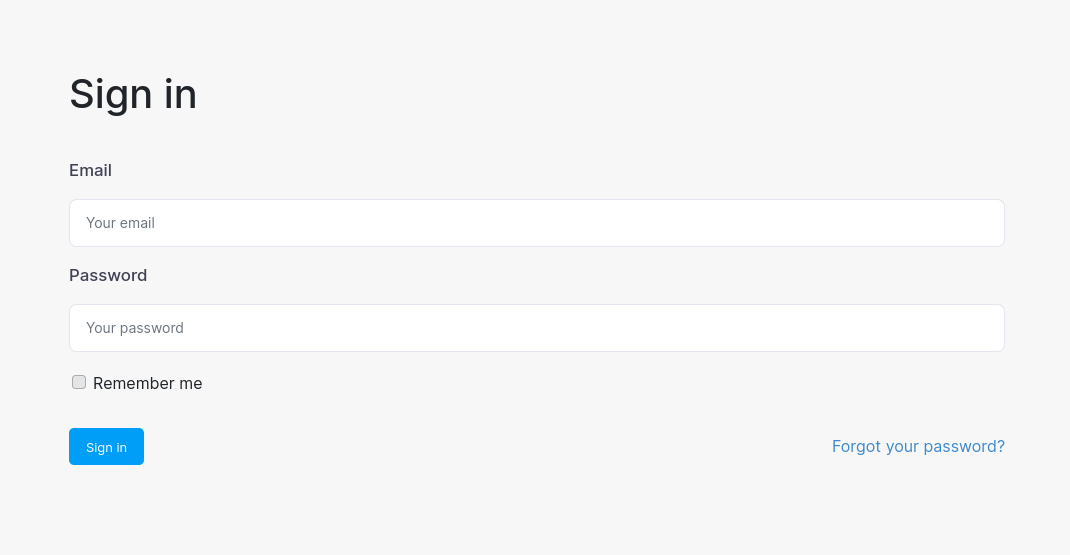
\includegraphics[width=\textwidth]{app/signin}
    \caption{Authentication page}
    \label{ss-signin}
\end{figure}

\subsection{Agents management page}
The figure \ref{ss-agents} illustrates the final result of the implementation of the agents management epic.
\begin{figure}[hbt!]
    \centering
    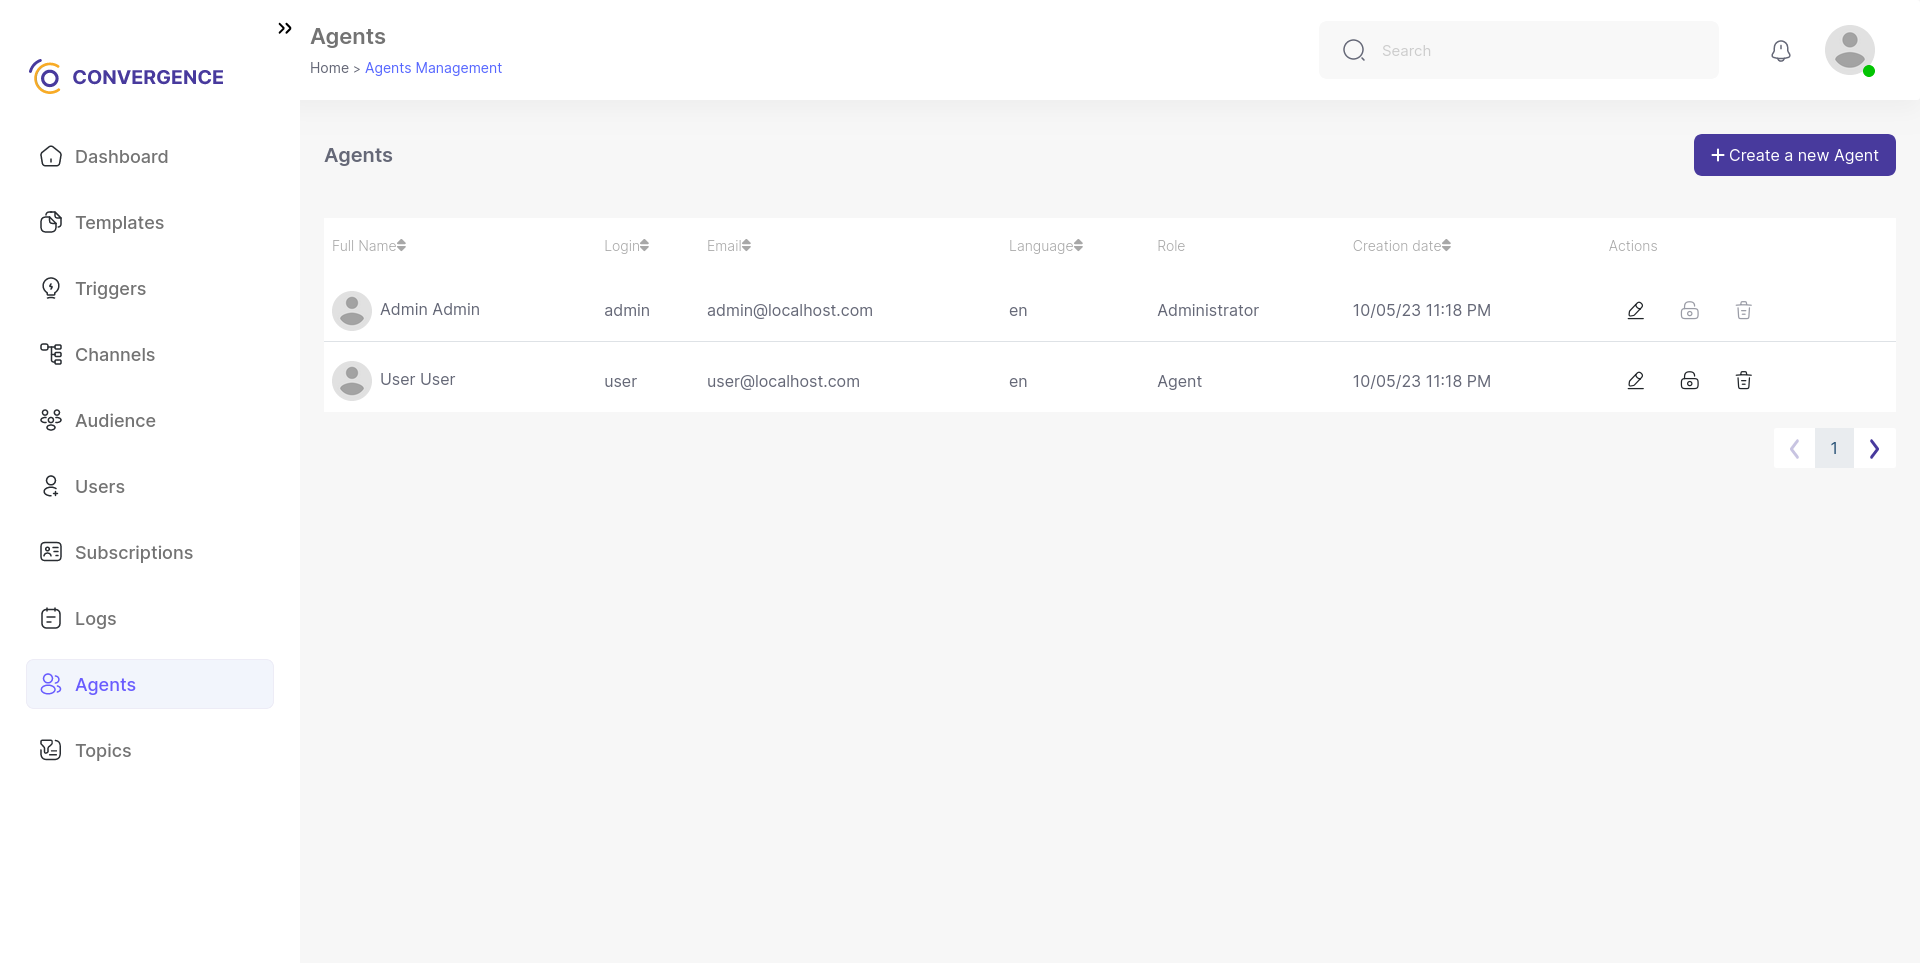
\includegraphics[width=\textwidth]{app/agents}
    \caption{Agents management page}
    \label{ss-agents}
\end{figure}

\subsection{Channels management page}
The figure \ref{ss-channels} illustrates the final result of the implementation of the channels management epic.
\begin{figure}[hbt!]
    \centering
    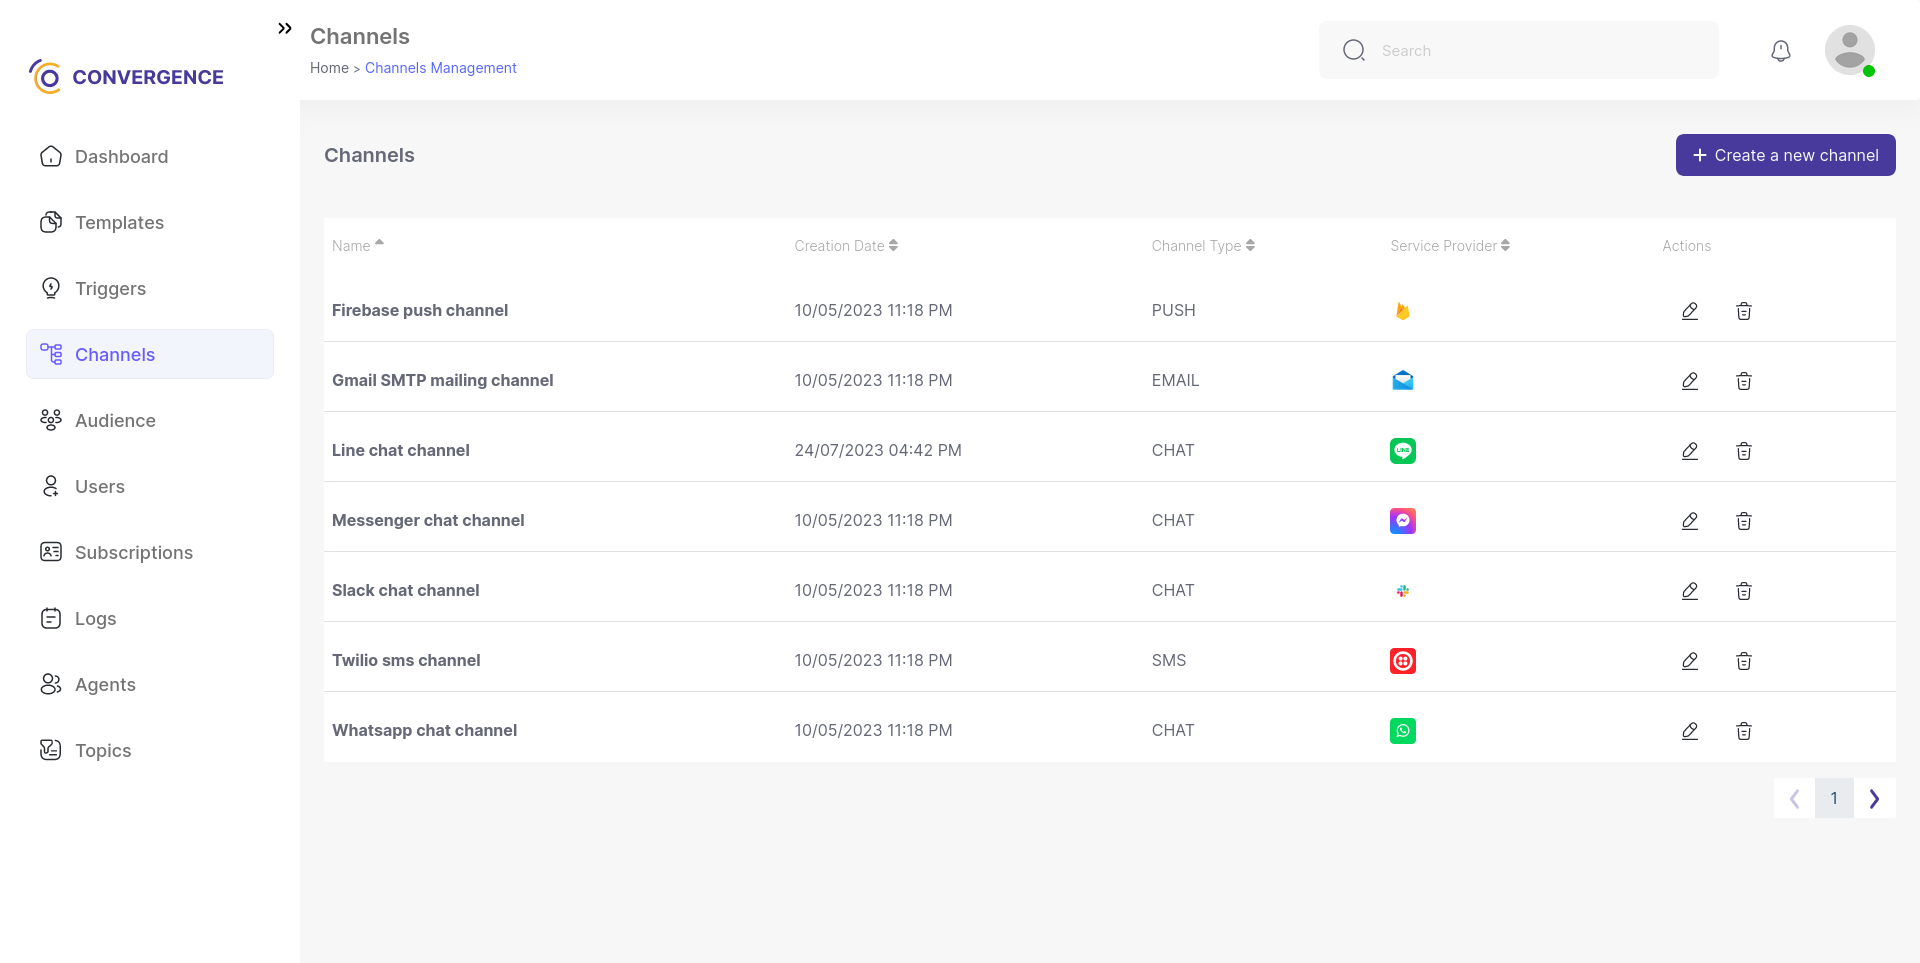
\includegraphics[width=\textwidth]{app/channels}
    \caption{Channels management page}
    \label{ss-channels}
\end{figure}

\phantomsection
\section*{Summary}
\addcontentsline{toc}{section}{Summary}